\documentclass{article}
\usepackage[utf8]{inputenc}
\usepackage{graphicx}
\usepackage{epstopdf}
\usepackage{caption}
\usepackage{subcaption}
\usepackage{multirow}
\usepackage{hyperref}
\usepackage{url}
\usepackage{seqsplit}
\hypersetup{pdfstartview={FitH null null null}}
\usepackage{amssymb,amsmath}
\usepackage{amsthm}
\usepackage{empheq}
\usepackage{algorithm,algpseudocode}
\usepackage[margin=1.5in]{geometry}
\usepackage{listings}
\lstset{language=Python} 

\usepackage{listings}
\usepackage{color} %red, green, blue, yellow, cyan, magenta, black, white
\definecolor{mygreen}{RGB}{28,172,0} % color values Red, Green, Blue
\definecolor{mylilas}{RGB}{170,55,241}


\title{Template based modeling using a homology-based algorithm}
\author{Xiaokai Qian, Sean Lander, Caiwei Wang, Haipei Fan, Puneet Gaddam, Brett Koonce\\University of Missouri - Columbia}

\date{Feburary 18, 2013}

\algloopdefx{NoEndIf}[1]{\textbf{If} #1 \textbf{then}}

\begin{document}

\maketitle

\section{Abstract}
We implement basic homology/template modeling of a DNA protein from CASP, T0644.  First, we search (BLAST), find the best candidate template, and align it with our target sequence.  Next, we build a copy of the the target protein's backbone using the template data wherever possible (our custom python tool).  Then, we refine our sidechains (SCWRL) to produce a candidate PDB.  Finally, we optimize (3D-Refine) our machine-generated model.  Ultimately, we visualize (JMOL) our results against the known structure of the protein and discuss how our method performs compared to others via objective functions (TM-Score/RMSD).

\section{Introduction}

Template modeling is an important technique in modern bioinformatics.  First, we begin with a DNA sequence of unknown structure.  By searching a database of known sequences, we can find similar proteins to our unknown target.  Then we can build a model of our target by using known elements from other proteins.\\\\
When the two sequences do not differ greatly, this approach can generate usable models far quicker than traditional methods (real-world x-ray crystal modeling can take years to produce a single structure).  However, this approach is not foolproof.  Of considerable importance is making sure that the differences between the between the two sequences are rectified, as well as making sure the final molecule is still a viable real-world model.\\\\
For our project, we implemented basic homology modeling in python, using a number of external tools to produce a pipeline capable of taking initial input sequence and presenting a final visualized model.



\subsection{Pipeline}
\begin{figure}[H]
\begin{center}
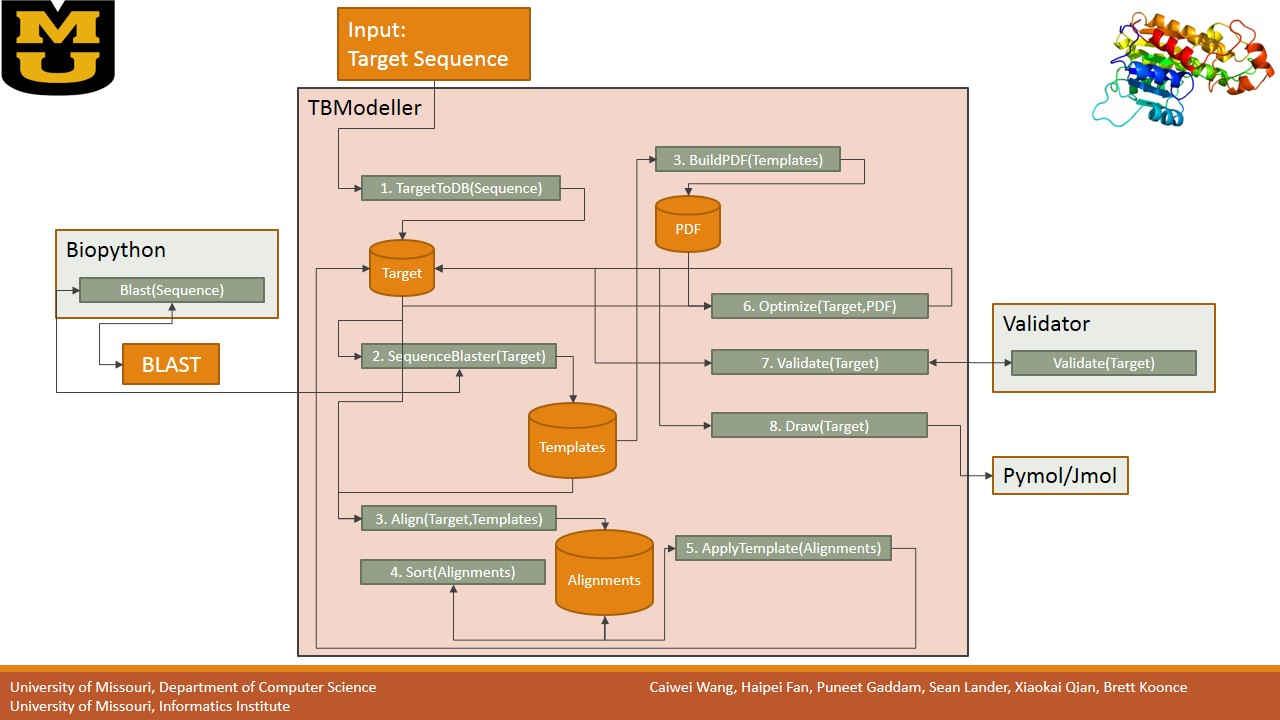
\includegraphics[width=\textwidth]{workflow}
\caption{An overview of the TBPy pipeline}
\label{Fig:blosum}
\end{center}
\end{figure}

\section{Template Search, Alignment and Data}

\subsection{CASP}

Critical Assessment of Techniques for Protein Structure Prediction (CASP) is a community-wide, worldwide experiment performed every two years since 1994, aiming to help improve the protein structure prediction techniques. The main goal of CASP is to evaluate the state-of-art in protein three-dimensional structure prediction, identify the advances that have been made, and pay close attention to future work that can be done. The methods of objective testing of these techniques have been provided through the process of blind prediction. It has been viewed more as a “world championship” in this field of science.\\

We selected some CASP targets (T0644, T0645, T0648) used in the 2012 modeling competition (which in turn means that we know what our eventual models should look like) and began our process.

\subsection{BLAST}

First, we take our input sequence and run it through the Basic Local Alignment Search Tool.  BLAST is a relatively time-efficient algorithm to compare amino-acid sequences of different proteins or the nucleotides of DNA sequences. BLAST can be used for inferring functional and evolutionary relationships between sequences as well as identifying members of gene families. The BLAST algorithm finds resembled sequences by locating short similar regions between two sequences using a heuristic approach. It compares a query sequence to a sequence database and computes the statistical significance of alignments to find sub-sequence in the database that resemble the query sequence within a certain threshold. The BLAST program is based on an open-source format and can be accessed freely over the internet. This enables anyone to be able to modify the code and implement similarity searches using the up-to-date datasets.\\

So, once we have run BLAST, we have a candidate template protein, as well as a sequence alignment between our search sequence and our template.

\subsection{PDB}

Next, for each target, we acquire the actual PDB file which describes the raw structure of the template DNA sequence.  The Protein Data Bank (PDB) is a repository for the collection, data processing and dissemination of the three-dimensional data on macromolecular structure, such as proteins and nucleic acids. The PDB is overseen by the Worldwide Protein Data Bank (wwPDB). It is a crucial resource for scientists nowadays who work in the area of structural biology as most major scientific journals require them to submit their data to the PDB. The structural data are commonly collected by X-ray crystallography or NMR spectroscopy and submitted by biologists and biochemists all over the world. These data can be freely and publically accessed by the global community on the Internet via the websites of its member organizations (PDBe, PDBj, and RCSB). 

\section{Building a protein}

The majority of the project centers around creating the structure of the target protein using the template files found in the previous steps. Using a template structure and its alignment with the target we are able to confidently create a structure for the target which is close to native.

\subsection{Algorithm - PDB to Structure}

The structure is created by using an alignment file and a structure file to create a structure for the target. Under optimal circumstances there will be no difference in length between the target and template. However this is not always the case, so it is important to pad the front and back of the template's alignment and structure with blank residues. This is recorded as a single dash, -, in the alignment and a triple dash, ---, in the structure. The structure is preprocessed and reduced down to a series of residues, each containing 4 atoms: N, CA, C, O. Residue names are changed from length 3 to length 1 so as to facilitate alignment checking between the template's alignment and structure.

\newpage
\subsection{Python - PDB to Structure}
\begin{lstlisting}
##NOTE: all calls to Atom in this code will need:
## ", missing=True" as a final argument, omitted for clarity
seq = []
curres = '---'
res = []
first = True
atomnum = 5
resnum = 0
for line in pdb.lines:
    # Decode from byte array
    line = line.decode()
    # Grab only ATOM lines
    if line[:6] == 'ATOM  ':
        # Get the atomname (N,CA,C,O)
        atomname = line[12:16]

        # First make sure you're only storing N, CA, C and O
        if atomname not in (' N  ',' CA ',' C  ',' O  ') \
		or line[16] not in (' ','A'):
            continue

        # Check to see if residue changed
        if line[17:20] != curres or atomnum > 4:
            if self.debug:
                print("%8s%8s%8s%8s" % ('CURRES','NEWRES','RESNUM','ATONUM'))
                print("%8s%8s%8d%8d" % (curres,line[17:20],resnum,atomnum))
                print(line)
            # Check to make sure the last residue was complete
            if atomnum < 5:
                # Add on the missing atoms to the end of the residue
                if atomnum == 1:
                    atom = Atom(atomName=' N  ',resName=curres,elemSym=' N')
                    res.append(atom)
                    atomnum += 1
                if atomnum == 2:
                    atom = Atom(atomName=' CA ',resName=curres,elemSym=' C')
                    res.append(atom)
                    atomnum += 1
                if atomnum == 3:
                    atom = Atom(atomName=' C  ',resName=curres,elemSym=' C')
                    res.append(atom)
                    atomnum += 1
                if atomnum == 4:
                    atom = Atom(atomName=' O  ',resName=curres,elemSym=' O')
                    res.append(atom)
                    atomnum += 1
            # Append the residue to the sequence
            if res: seq.append((amino3to1[curres],res))

            # If this is the first atom fill in the blanks from the PDB
            if first:
                first = False
                if self.debug:
                    print("Starting resnum:",int(line[22:26]))
                # Residue number of first residue in PDB
                for k in range(1,int(line[22:26])):
                    resname = '---'
                    res = []
                    res.append(Atom(atomName=' N  ',resName=resname,elemSym=' N'))
                    res.append(Atom(atomName=' CA ',resName=resname,elemSym=' C'))
                    res.append(Atom(atomName=' C  ',resName=resname,elemSym=' C'))
                    res.append(Atom(atomName=' O  ',resName=resname,elemSym=' O'))
                    seq.append((amino3to1[resname],res))
                # Decrement resnum by one to mimic the last res not in the PDB
                resnum = int(line[22:26])-1

            # Check for resnum increment so we don't miss residues
            resinc = int(line[22:26])-resnum
            if resinc != 1:
                if self.debug:
                    print("Resiude skip:",resnum,"->",int(line[22:26]))
                for k in range(1,resinc):
                    resname = '---'
                    res = []
                    res.append(Atom(atomName=' N  ',resName=resname,elemSym=' N'))
                    res.append(Atom(atomName=' CA ',resName=resname,elemSym=' C'))
                    res.append(Atom(atomName=' C  ',resName=resname,elemSym=' C'))
                    res.append(Atom(atomName=' O  ',resName=resname,elemSym=' O'))
                    seq.append((amino3to1[resname],res))

            # Reset the residue
            res = []
            # Store residue numbers
            resnum = int(line[22:26])
            # Store the atom number
            atomnum = 1

        # Make sure current residue name is set
        curres = line[17:20]

        '''
        if self.debug:
            print("Line:",line)
        '''

        # Check to make sure the right atom is being stored
        if atomnum == 1:
            if atomname != ' N  ':
                atom = Atom(atomName=' N  ',resName=curres,elemSym=' N')
                res.append(atom)
                atomnum += 1
        if atomnum == 2:
            if atomname != ' CA ':
                atom = Atom(atomName=' CA ',resName=curres,elemSym=' C')
                res.append(atom)
                atomnum += 1
        if atomnum == 3:
            if atomname != ' C  ':
                atom = Atom(atomName=' C  ',resName=curres,elemSym=' C')
                res.append(atom)
                atomnum += 1
        if atomnum == 4:
            if atomname != ' O  ':
                atom = Atom(atomName=' O  ',resName=curres,elemSym=' O')
                res.append(atom)
                atomnum += 1
                continue
        if atomnum > 4:
            continue
        # Store off the atom information if valid
        atom = Atom(
            atomName=atomname,
            altLoc=line[16],
            resName=line[17:20],
            chainId=line[21],
            codeForInsertion=line[26],
            xcoord=float(line[30:38]),
            ycoord=float(line[38:46]),
            zcoord=float(line[46:54]),
            occ=float(line[54:60]),
            temp=float(line[60:66]),
            elemSym=line[76:78],
            charge=line[78:80]
        )
        # And add it to the residue (in the proper order)
        res.append(atom)
        atomnum += 1

# Add the final residue to the sequence
seq.append((amino3to1[curres],res))
\end{lstlisting}

\newpage
\subsection{Algorithm - Structure to PDB}

Once the preprocessing is complete the alignment and structure can be used to create the target's structure.

\subsection{Python - Structure to PDB}

\begin{lstlisting}
## target = [residue], template = [residue]
## structure = [(residueName,residue)]
BuildStructure(target,template,structure):
    i,j = 0
    target_structure = []
    while i < length(target) and j < length(structure):
        # template[i] in alignment is blank
        if template[i] == ‘-‘:
            # create a residue with blank atoms
            res = BlankResidue()
            target_structure.append(res)
            i++
            # structure file missing residue
            if structure[j][0] == ‘-‘:
                j++
            continue
        # target[i] in alignment is blank
        if target[i] == ‘-‘:
            i++, j++
            continue
        # copy the atoms
        res = copyAtoms(structure[j][1])
        # change the residue name for atoms
        changeResidueName(res,target[i])
        target_structure.append(res)
        i++, j++
    
    final_structure = []
    for res in target_structure:
        for atom in res:
            if not atom.blank:
                 final_structure.append(atom)
\end{lstlisting}


\section{Optimization and sidechains}

\subsection{SCWRL}

Finally, we run our candidate PDB file through SCWRL, a program for adding sidechains to a protein backbone.  SCWRL4 is based on an improved graph theory algorithms that solve the combinatorial problem in side-chain prediction more rapidly than many other available programs.\\

SCWRL4 is based on a new potential function that results in improved accuracy at reasonable speed.It will converge on very large proteins or protein complexes or those with very dense interaction graphs.It depends on a backbone-dependent rotamer library. The library provides lists of chi1-chi2-chi3-chi4 values and their relative probabilities for residues at given phi-psi values, and explores these conformations to minimize sidechain-backbone clashes and sidechain-sidechain clashes.\\

The SCWRL4 executable saves the resolved optimal conformation of the whole protein model into PDB file. The corresponding value of the total energy is printed into the standard output, which can be redirected to a file for further analysis.

\subsection{3DRefine}

Next, we used a two-step refinement protocol, called 3Drefine, to consistently bring the initial model closer to the native structure.  One of the major limitations of computational protein structure prediction is the deviation of predicted models from their experimentally derived true, native structures.  The first step is based on optimization of hydrogen bonding (HB) network and the second step applies atomic-level energy minimization on the optimized model using a composite physics and knowledge-based force fields. The approach has been evaluated on the CASP benchmark data and it exhibits consistent improvement over the initial structure in both global and local structural quality measures. 3Drefine method is also computationally inexpensive, consuming only few minutes of CPU time to refine a protein of typical length (300 residues).

\section{Visualization}

After we obtain final target PDB file, we use Jmol to visualize it. At the same time, we also visualize the native one to compare it with our prediction.  The left one is a target structure we generated (T0644), while right one is the native structure.

\subsection{Visualizations}

\begin{figure}
\centering
\begin{minipage}{.5\textwidth}
  \centering
  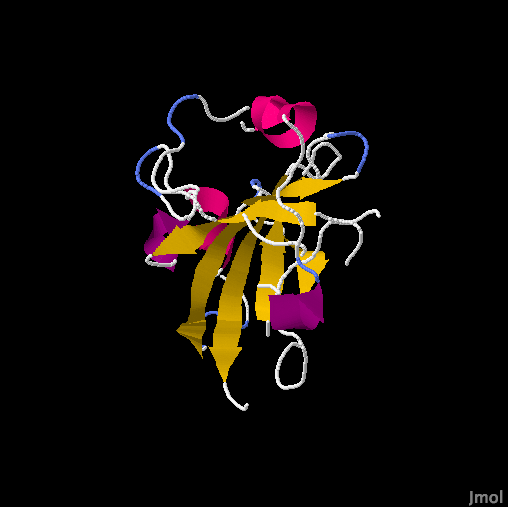
\includegraphics[width=.9\linewidth]{target_group}
  \captionof{figure}{Target structure}
  \label{fig:test1}
\end{minipage}%
\begin{minipage}{.5\textwidth}
  \centering
  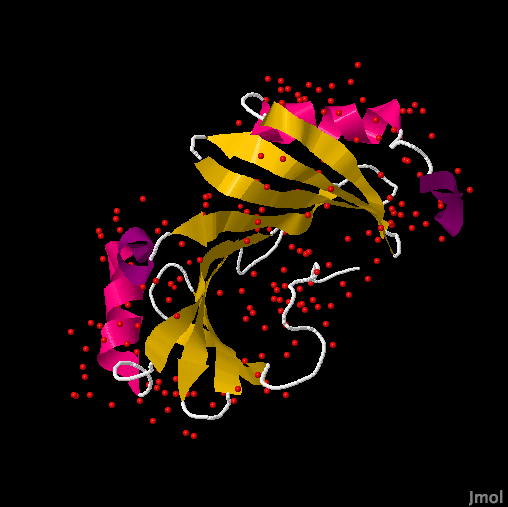
\includegraphics[width=.9\linewidth]{target_native}
  \captionof{figure}{Native structure}
  \label{fig:test2}
\end{minipage}
\end{figure}

\section{Results}

After we generated the target PDB file, we use TM-Score and RMSD to evaluate our prediction. Also we compared our prediction with other servers’ results based on same target. In our project, we choose MuFold and MULTICOM to compare our results.\\\\
TM-score is an algorithm to calculate the structural similarity of two protein models. It is often used to quantitatively assess the accuracy of protein structure predictions relative to the experimental structure. Because TM-score weights the close atom pairs stronger than the distant matches, it is more sensitive to the topology fold than the often-used root-mean-square deviation (RMSD) since a local variation can result in a high RMSD value. TM-score has the value in (0,1). Based on statistics, a TM-score \textless0.17 corresponds to a random similarity and a TM-score \textgreater0.5 generally corresponds to the same fold in SCOP/CATH. The definition of TM-score is independent on the length of the proteins.\\\\
RMSD is the measure of the average distance between the atoms (usually the backbone atoms) of superimposed proteins. In the study of globular protein conformations, one customarily measures the similarity in three-dimensional structure by the RMSD of the Cα atomic coordinates after optimal rigid body superposition.\\\\
Our results are shown in the following table. From the table, it would appear that our results are comparable with both MULTICOM and MuFold. But, we have only tried one target we have tried (and tweaked our algorithm to look closer to the end goal, which we knew before). In the future, we should try this approach on some unknown proteins.  But, these metrics provide an interesting objective metric of our predictions.

\subsection{Scores}
\begin{center}
    \begin{tabular}{ | l | l | l | p{2cm} |}
    \hline
      & Group1 & MULTICOM & MuFold \\ \hline
    TM-Score & 0.9992 & 0.9072 & 0.1985 \\ \hline
    RMSD & 0.118 & 1.666 & 14.978 \\
    \hline
    \end{tabular}
\end{center}

\section{Citations}

We thank the following tools and papers: \\\\

Cock PJ, Antao T, Chang JT, Chapman BA, Cox CJ, Dalke A, Friedberg I, Hamelryck T, Kauff F, Wilczynski B, and de Hoon MJ. Biopython: freely available Python tools for computational molecular biology and bioinformatics. Bioinformatics 2009 Jun 1; 25(11) 1422-3.\\\\

Blast:  Altschul S.F., Gish W., Miller W., Myers E.W. and Lipman D.J. (1990)
Basic local alignment search tool.  J. Mol. Biol. 215: 403-410.\\\\

CASP: Critical Assessment of Techniques for Protein Structure Prediction.\\
http://predictioncenter.org/casp10/ \\\\

PDB ID: 102l.
D.W.Heinz, W.A.Baase, F.W.Dahlquist, B.W.Matthews, "How Amino-Acid Insertions are Allowed in an Alpha-Helix of T4 Lysozyme," Nature, 361 (1993): 561.\\\\

D. Bhattacharya and J. Cheng: 3Drefine: Consistent Protein Structure Refinement by Optimizing Hydrogen-Bonding Network and Atomic-Level Energy Minimization.
Proteins: Structure, Function and Bioinformatics. 2012 (In Press).\\\\

G. G. Krivov, M. V. Shapovalov, and R. L. Dunbrack, Jr. Improved prediction of protein side-chain conformations with SCWRL4. Proteins (2009).\\\\

Jmol: an open-source Java viewer for chemical structures in 3D. http://www.jmol.org/ \\\\

Y. Zhang, J. Skolnick, Scoring function for automated assessment of protein structure template quality, Proteins, 2004 57: 702-710
J. Xu, Y. Zhang, How significant is a protein structure similarity with TM-score=0.5? Bioinformatics, 2010 26, 889-895\\\\

Hurley JR and Cattell RB (1962). "The Procrustes Program: Producing direct rotation to test a hypothesized factor structure". Behavioral Science 7 (2): 258–262.\\\\

Petitjean M (1999). "On the Root Mean Square quantitative chirality and quantitative symmetry measures". Journal of Mathematical Physics 40 (9): 4587–4595\\\\

\end{document}


\end{document}
